Aquí mostraremos la temperatura ambiente a la placa Arduino directamente en el
display LCD, sin comunicarse con otros dispositivos. El montaje es el que
sigue:

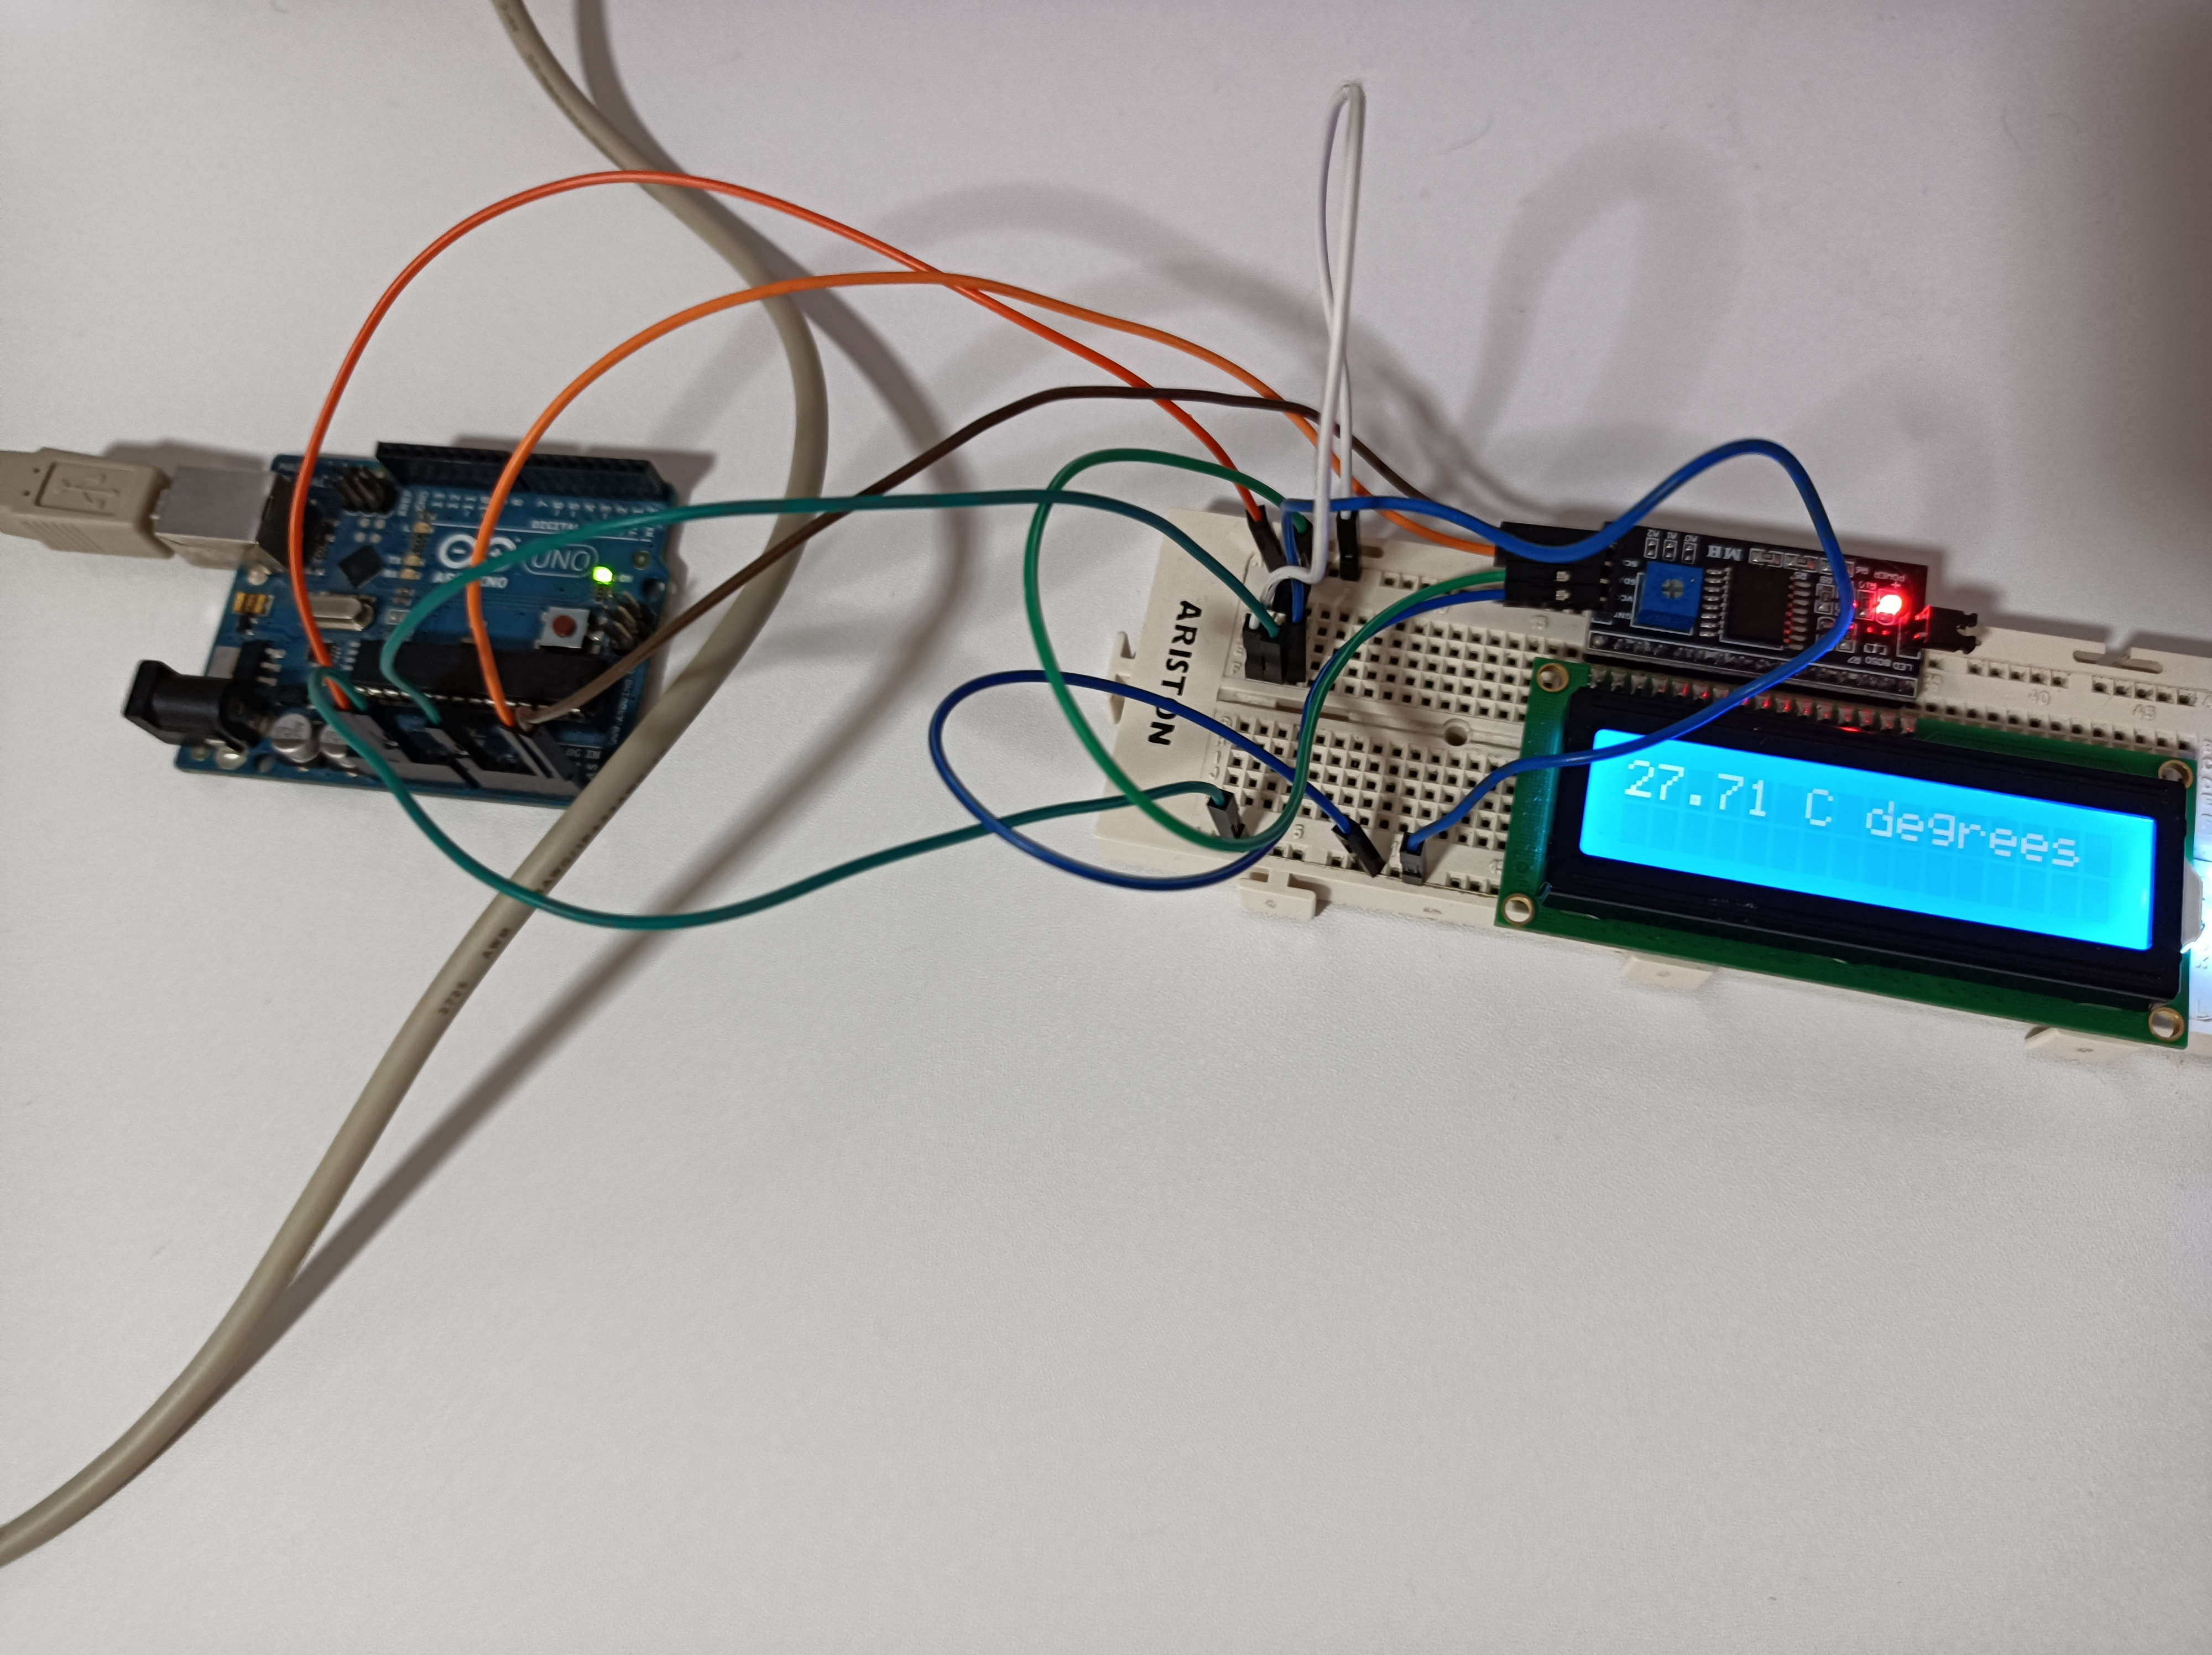
\includegraphics[width=\linewidth]{temperature-display-wiring.jpg}

Para traducir las mediciones de tensión en cifras de temperatura hay que
aplicar la siguiente fórmula:

\begin{equation*}
T = 100V - 50
\end{equation*}

Donde $V$ es la medición en \emph{voltios} y $T$ la cifra de temperatura.

Esto a su vez requiere traducir la medición numérica de la entrada analógica en
una cifra que refleje la magnitud en \emph{voltios}. Esta es la expresión que
define esta transformación:

\begin{equation*}
V = \frac{D}{D_{max}} \cdot V_{max}
\end{equation*}

Donde $D$ es la lectura conseguida, $V_{max}$ la tensión máxima que soporta el
pin analógico (que en este caso son \emph{5 V}) y $D_{max}$ la lectura máxima
que puede devolver el puerto (que en este caso es \emph{1023}).

Con esta información y la librería \verb|LiquidCrystal_I2C|\footnotemark, así
se programaría la placa Arduino para cumplir el propósito establecido:

\footnotetext{\url{
    https://github.com/johnrickman/LiquidCrystal_I2C/archive/refs/tags/1.1.3.zip
}}

\lstinputlisting[language=C++, caption=temperature-display.ino]{
    1/temperature-display/temperature-display.ino
}